\chapter{Accelerating Convolutional Neural Networks for FPGA using Depthwise Separable Convolution and Pruning} \label{chap:pratique}
%
%
In the previous chapter, we have introduced pruning, which can reduce both the size and the computational complexity of a \acrshort{cnn}. We have also seen that there exist various pruning schemes. Each of them can be categorized from coarse grained to fine-grained. Coarse-grained pruning schemes have the advantage of being easily implemented on \acrshort{gpu} and \acrshort{cpu} in exchange for a drop of accuracy. On the opposite, fine-grained pruning schemes have better accuracy but creates irregular access pattern that makes them difficult to implement. To have an efficient \acrshort{fpga}-based architecture, we should focus on implementing the most fine-grained pruning possible in order to have a higher sparsity and limit the drop of accuracy. Moreover, the pruning scheme should be done in such a way that is not easily implementable on \acrshort{gpu} and \acrshort{cpu} to make it relevant on \acrshort{fpga}.

In order to further reduce the number of weights and operations, we will define a\acrshort{fpga}-based architecture that integrates both pruning and \acrshort{dsc}. The objectives of the architecture and its associated pruning scheme are the following:
%
\begin{itemize}
    \item The pruning scheme reduces the computational complexity.
    \item The pruning scheme allows a reduction of the memory required to store the weights.
    \item The pruning scheme must be the least coarse-fined.
    \item An increase of the sparsity does not degrade the performance of the architecture.
\end{itemize}
%
First, Section \ref{sec:design} aims at developping the pruning scheme and the dataflow to handle it. We then perform a loop analysis.

Second, Section \ref{sec:implementation} describes the \acrshort{fpga}-based architecture performing the dataflow detailed at previous section.

Third, Section \ref{sec:measure} shows the results obtained and discusses the limits of the implementation.
%
%
\section{Design of an FPGA-based accelerator integrating structured sparse DSC} \label{sec:design}
As previously said,  the aim of this section is to develop a pruning scheme for \acrshort{cnn} model (MobileNetV2) and a dataflow able to support it. First we details the pruning scheme used and the gain obtained by applying the pruning. 
%
\subsection{Pruning scheme} \label{subsec:pscheme}
%
\acrshort{dsc} is composed of two types of convolution: depthwise and pointwise convolution. We have decided to apply pruning on the pointwise filters for various reasons:
%
\begin{itemize}
    \item In MobileNet and MobileNetV2, most of the operations are done in the pointwise convolutions \cite{zhang_channel_2019, tu_pruning_2019}.
    \item As each kernel of pointwise kernel, is a vector of size $1 \times 1  \times Nif$. It means that we have to prune in the axis of the channel and apply the same scheme as \textcite{kang_accelerator-aware_2020}.
    \item As in MobileNetV2, each \acrshort{dsc} follows a $1 \times 1$ convolution, we can apply the pruning scheme to every $1 \times 1$ convolutions in the network.
\end{itemize}
%
As mentionned above, we can develop a pruning scheme that is inspired by the methodology of \textcite{kang_accelerator-aware_2020} which performs an channel-axis pruning. Ideally, without pruning, each \acrshort{pe} performing a pointwise convolution, fetches $N_{if}$ weights and their corresponding input pixels (pointwise convolution only convolve pixels in the channel-axis). Then each non-pruned weight is convolved with its corresponding pixel. However, as the resource of the \acrshort{fpga} are limited, the \acrshort{pe} can load $N_{par} \leq N_{if}$ weights and pixels.

%
\begin{figure}
    \centering
    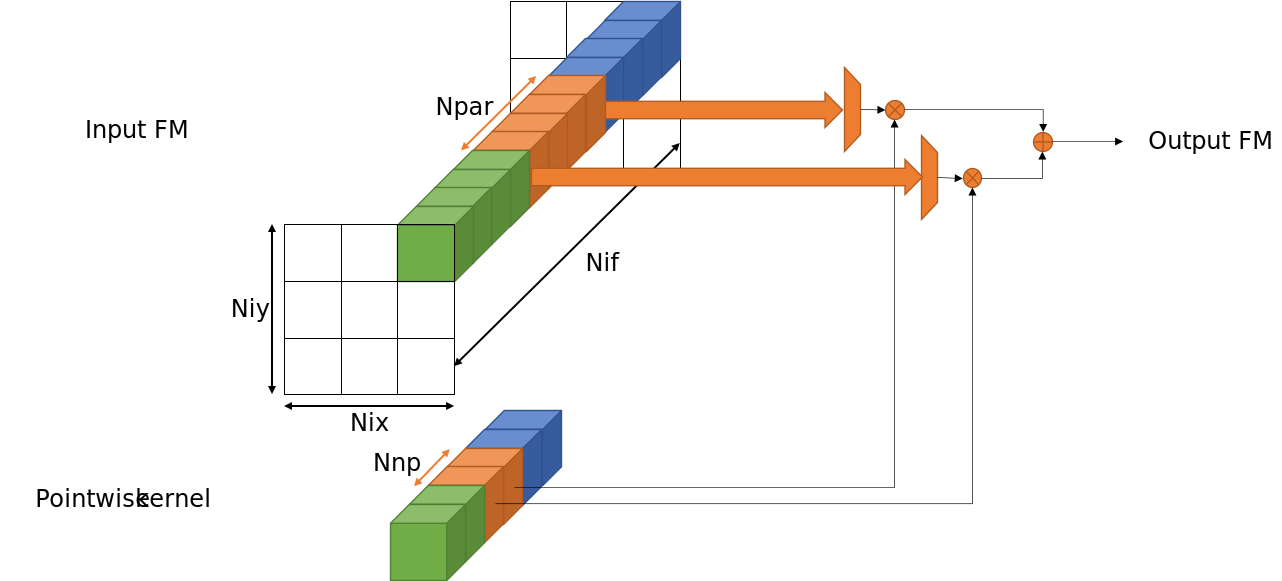
\includegraphics[width=\textwidth]{pruningscheme.pdf}
    \caption{Process of convolution with a sparse pointwise kernel, inspired from \cite{kang_accelerator-aware_2020}}
    \label{fig:prunedwg}
\end{figure}
%
As pointed out by \cite{kang_accelerator-aware_2020}, the unstructured pruning of the pointwise kernel can cause several issues. First, it can causes misalignement between the weight and pixel fetching group. Indeed if we prune the first $N_{par}$ weights in the kernel, the first pixels fetching is useless. Second, there can be a load-imbalance problem that can occur between two \acrshort{pe}s if the number of weights between the two kernels is different. To solve these problems, the solution proposed by \cite{kang_accelerator-aware_2020} is to allign fetching groups of size $N_{par}$, and for each weight fetching group keep a uniform number of weights called $N_{np}$, as illustrated in Figure \ref{fig:prunedwg}. Therefore, it solves also the load imballance problem and can be applied to every $1 \times 1$ kernels.

%
\begin{table}
    \center
    \begin{tabular}{|c|c|c|}
        \hline
        $N_{par}$ & The input pixel fetching group size. & $N_{par} \leq N_{if}$ \\
        \hline
        $N_{np}$  & The pointwise weight fetching group size. & $N_{np} \leq N_{par}$ \\
        \hline
        $N_{gr}$  & The number of fetching groups & $N_{gr} = \left\lceil \frac{N_{if}}{N_{par}} \right\rceil $ \\
        \hline
        $\alpha$  & The pruning ratio & $\alpha = \frac{N_{np}}{N_{par}}  $ \\
        \hline
    \end{tabular}
    \caption{Pruning parameters}
    \label{tab:pr_param}
\end{table}
%
To summarise, each depthwise kernel is composed of $N_{gr}$ weight fetching groups of $N_{np}$ weights, where each group corresponds to a pixels fetching group of size $N_{par}$. We should add that this pruning scheme is not the same as \textit{channel pruning} since we do not constraint the same weights to be pruned in each group. Therefore, I have not considered the pruning of the pointwise filter associated with the pruning of a weight in each kernels. The pruning parameters are defined in Table \ref{tab:pr_param}.
%
\subsubsection{Reduction factor}
%
We can now evaluate the reduction factor of the \acrshort{dsc} including pruning with respect to the \acrshort{dsc} without pruning and the standard convolution. Considering the size of the input feature map of the pointwise convolution is $N_{ix}  \times N_{iy} \times N_{if}$, the size of the depthwise filter is $N_{kx} \times N_{ky} \times N_{if}$, the size of the non-pruned pointwise convolution $N_{if} \times N_{of}$, the fetching group size is $N_{par}$, and the number of pruned weights is $N_{np}$. The amount of weights $W_{DSC}$ and operations $O_{DSC}$ of the \acrshort{dsc} can be determined using Equation \eqref{eq:dsc_wg_op} \cite{bai_cnn_2018, liu_fpga-based_2019}.
%
\begin{align}
    W_{DSC} &= N_{kx} \times N_{ky} \times N_{if} + N_{if} + \times N_{of}\\
    O_{DSC} &= N_{ix} \times N_{iy} \times N_{kx} \times N_{ky} \times N_{if} + N_{ix} \times N_{iy} \times N_{if} \times N_{of}
    \label{eq:dsc_wg_op}
\end{align}
%
The same way, the amount of weights $W_{PR_DSC}$ and operations $O_{PR_DSC}$ of the \acrshort{dsc} with pruning can be determined using Equation \eqref{eq:pr_dsc_pr_wg_op}.
%
\begin{align}
    W_{PR_DSC} &= N_{kx} \times N_{ky} \times N_{if} + \times N_{if} + N_{np} \times N_{gr} \times N_{of}\\
    O_{PR_DSC} &= N_{ix} \times N_{iy} \times N_{kx} \times N_{ky} \times N_{if} + N_{ix} \times N_{iy} \times N_{gr} \times N_{np} \times N_{of} 
    \label{eq:pr_dsc_wg_op}
\end{align}
%
Thus, the reduction factor on weights $F_{Wg}$ and operations $F_{Op}$ can be calculated in Equation \eqref{eq:factor_comp}. More information about the demonstration to find the relations can be found in Appendix \ref{appendix:factor}.
%
\begin{align}
    F_{Wg} &= \frac{1 + \frac{N_{kx} \times N_{ky}} {N_{of}}} {\alpha + \frac{N_{kx} \times N_{ky}} {N_{of}}}\\
    F_{Op} &= \frac{1 + \frac{N_{kx} \times N_{ky}} {N_{of}}} {\alpha + \frac{N_{kx} \times N_{ky}} {N_{of}}}
    \label{eq:factor_comp}
\end{align}
%
\begin{figure}
    \centering
    \includegraphics[width=\textwidth]{RedFactor.pdf}
    \caption{Evolution of the reduction factor depending on the pruning ratio and the number of output channel}
    \label{fig:redfacto}
\end{figure}
%
As the reduction factor depend on the pruning ratio $\alpha$, we can illustrate the evolution of the reduction factors depending on this parameter and on the different $N_{of}$ of the network. This can be seen on Figure \ref{fig:redfacto}. For example, if we apply a pruning ratio of $75\%$, the reduction factors with respesct to the \acrshort{dsc} without pruning are between two and four times. If we consider the reduction factor between \acrshort{dsc} and standard convolution to be 9 times, the reduction factors between proposed \acrshort{dsc} and standard convolution is between 18 and 36 times
%
\subsubsection{Compressed format}
%
\begin{figure}
    \centering
    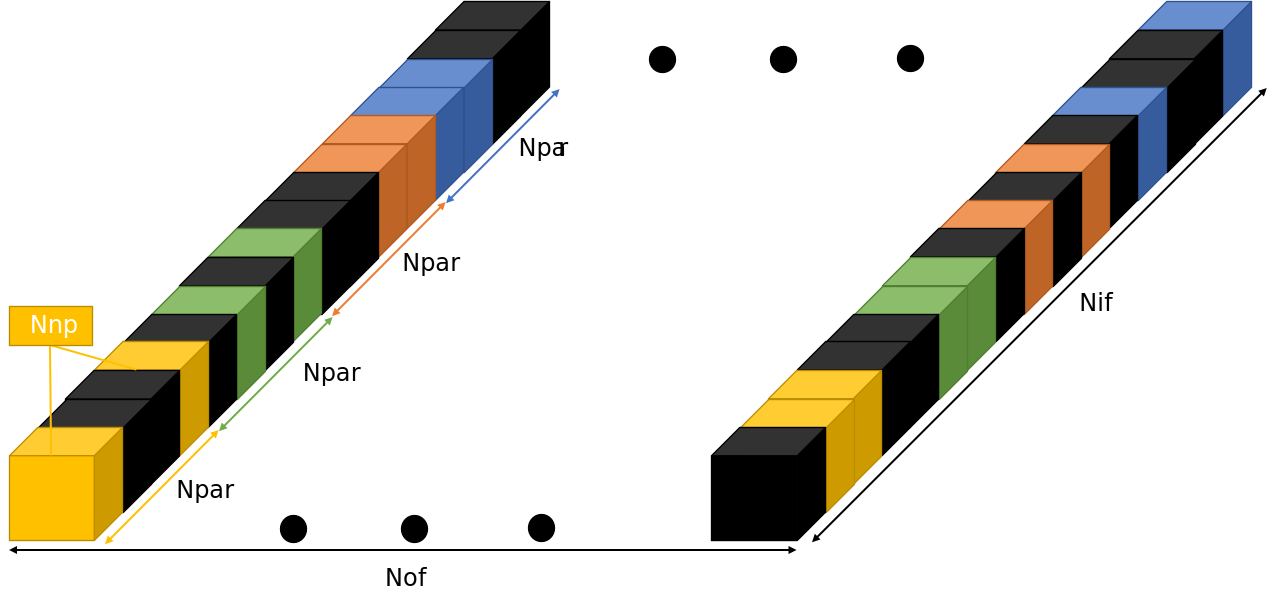
\includegraphics[width=\textwidth]{pruned_wg.pdf}
    \caption{A pointwise kernel after pruning}
    \label{fig:pruned_wg}
\end{figure}
%
After applying the pruning scheme on the pointwise kernels, the kerels become sparse and it means that is contains a lot of 0 value weights, as illustrated in Figure \ref{fig:pruned_wg}. Therefore, in order to reduce the memory usage, we should store the non-pruned weights in a compressed format that allow to find the address of the weight with no extra-overhead.

A conventional storage formats for sparse matrix is the \acrfull{csr} \cite{buluc_parallel_2009}. According to \textcite{buluc_parallel_2009}, \textquote{\textit{The compressed sparse row (CSR) format stores the nonzeros (and ideally only the nonzeros) of each matrix row in consecutive memory locations,  and  it  stores  an  index  to  the  first  stored  element of each row}}. In other words, we represent a sparse matrix using three vectors:
%
\begin{itemize}
    \item \textbf{Vector val}: containing all the values of the non-pruned weights.
    \item \textbf{Vector col\_ind}: contains the column indices of the elements in \textbf{val}.
    \item \textbf{Vector row\_ptr}: contains the index of each row in \textbf{val}.
\end{itemize}
%
However, as for \cite{zhu_efficient_2020}, this format can be compressed further thanks to the pruning scheme. Indeed, since the kernels to compress are vectors, we can reduce the storage usage by removing the \textbf{row\_ptr} vector. Moreover, we have a better compression if we reduce the number of bits allocated to represent the column index of a weigth. Indeed, knowing that the weight correpond to a pixel in a fetching group of size $N_{par}$, we can only save the position of the pixel in that group. As a result, we can reduce the number of bits from $log_2(N_{if})$ to $log_2(N_{par})$, where $N_par \leq N_{if}$.

%
\begin{figure}
    \centering
    \includegraphics[width=\textwidth]{MinCompr.pdf}
    \caption{Minimal pruning ratio if $BW$ = 16}
    \label{fig:prun_mem}
\end{figure}
%
As this compressed format requires an extra vector, we compute the minimal pruning ratio required to have a reduction of the memory usage. The relation between minimal pruning ratio and memory reduction ca be found in Equation \eqref{eq:prun_mem} where $BW$ is the bitwidth required to represent the value of a weight. The curve representing the minimal pruning ratio depending on $N_{par}$ is illustrated in Figure \ref{fig:prun_mem}. We can conclude that we need at least a pruning ration of $40\%$ in order to save memory (a fewer pruning ratio can be set if we have a small $N_{par}$).
% 
\begin{equation}
    \alpha < \frac{BW}{ BW + log_2(N_{par})}
    \label{eq:prun_mem}
\end{equation}
%
\subsection{Adding the pruning scheme to MobileNetV2}
%
As we have seen how the weights of a $1 \times 1$ kernel are pruned and the compressed format of the kernels, we explain in this section how to integrate the proposed pruning scheme into the \acrshort{dsc}. In MobileNetV2, the \acrshort{dsc} layer is included into a larger building block, the \textit{inverted residual block} (see Section \ref{subs:mbv2}). It means that the \acrshort{dsc} follows a $1 \times 1$ convolution layer that expands the number of channel. As a result, we have to compute two sparse $1 \times 1$ convolutions. 

%
\begin{figure}
    \centering
    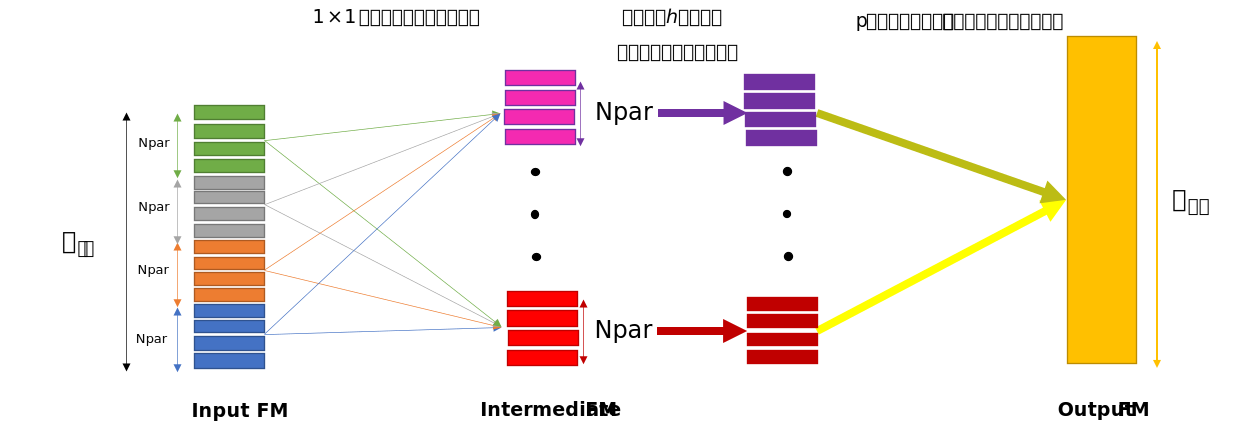
\includegraphics[width=\textwidth]{algo.pdf}
    \caption{Illustration of the algorithm used to perfom the convolutions}
    \label{fig:algo}
\end{figure}
%
As explained in Section \ref{subsec:pscheme}, each $1 \times 1$ convolution has to fetch $N_{par}$ input pixels, which corresponds to $N_{par}$ channels. Consequently, if the expansion $1 \times 1$ convolution produces $N_{par}$ channels, the \acrshort{dsc} can fetches those intermediate products and produces partial results of the output \acrshort{fm}. Indeed, we can first perform the depthwise convolution with each intermediate channel and then performing the partial pointwise convolution with the corresponding weight in each pointwise kernel, as illustrated in Figure \ref{fig:algo}. The block has finished when it has performed the previous steps for each intermediate group. This approach has been chosen, instead of producing directly each final output result, to reuse at most the products of the $1 \times 1$ convolution.

\begin{algorithm}[H]
    \centering
    \begin{algorithmic}
        \For{$group_{int}:=0$; $group_{int} < Ngr_{int}$; $group_{int}++$}
            \State{1*1\_convolution ($group_{int}$)}
            \State{DSC($group_{int}$);}
        \EndFor
    \end{algorithmic}
    \caption{Pseudocode of the algorithm}
    \label{pseudocode:overal_pseudo_code}
\end{algorithm}
%
We can translate this algorithm into a pseudocode, observed at Figure \ref{pseudocode:overal_pseudo_code}, where $group$ (respect. $group_{int}$) is the index of fetching group in the input \acrshort{fm} (resp. intermediate \acrshort{fm}, since the number of input channels is expanded by a factor $t$) and $Ngr_{int} = \left\lceil \frac{N_{if} \times t}{N_{par}} \right\rceil$ is the number of intermediate fetching group. We can now detail how each convolution is going to be performed:
%
%
\begin{enumerate}
    \item \textbf{1*1\_convolution}: We have to fetch the $N_{par}$ kernels corresponding to the \acrshort{dsc} fetching group. Indeed, the \acrshort{dsc} fetches $N_{par}$ channels corresponding to a spatial position $(intx, inty)$ of the intermediate \acrshort{fm}. Then we can perform the convolution. As described in Section \ref{subs:2dconv}, the kernel acts a sliding window on the input \acrshort{fm}. For each pixel at position $(ix, iy)$, the convolution loads iteratively each weight and pixel fetching group. For each fetching group $group \leq N_{group}$, the convolution is performed by multiplying each non-pruned weight with its corresponding channel and accumulates it with the result of the previous group. The process is finished when the $N_{par}$ intermediate \acrshort{fm} channels have been produced (of size $N_{ix} \times N_{iy}$). The corresponding pseudocode is found in Algorithm \ref{pseudocode:c11} and the process is shown in Figure \ref{fig:algo_11conv}.
    \begin{algorithm}[H]
        \centering
        \begin{algorithmic}
            \For{$int_{f}:=0$; $int_{f} < N_{par}$; $int_{f}++$} \Comment{Loop 3}
                \For{$int_{x}:=0$; $int_{x} < N_{ix}$; $int_{x}++$} \Comment{Loop 2}
                    \For{$int_{y}:=0$; $int_{y} < N_{iy}$; $int_{y}++$} \Comment{Loop 2}
                        \For{$group:=0$; $group < N_{gr}$; $group++$} \Comment{Loop 1}
                            \For{$i_f:=0$; $i_f < N_{np}$; $i_f++$} \Comment{Unrolled}
                                \State{$wgt$  = $filter_{1 \times 1}$[$group_{int} \times N_{par} + int_f$][$group \times N_{par} + i_f$]}
                                \State{$acti$  = $FMI_{I}$[$wgt[pos] + group \times N_{par}$][$int_y$][$int_x$]}
                                \State{FM$_{int}$[$group_{int} \times N_{par} + int_f$][$int_y$][$int_x$]  += $acti \times wgt[val]$}
                            \EndFor
                        \EndFor
                    \EndFor
                \EndFor
            \EndFor
        \end{algorithmic}
        \caption{Sparse $1 \times 1$ convolution pseudocode}
        \label{pseudocode:c11}
    \end{algorithm}
    %
    \begin{figure}[H]
        \centering
        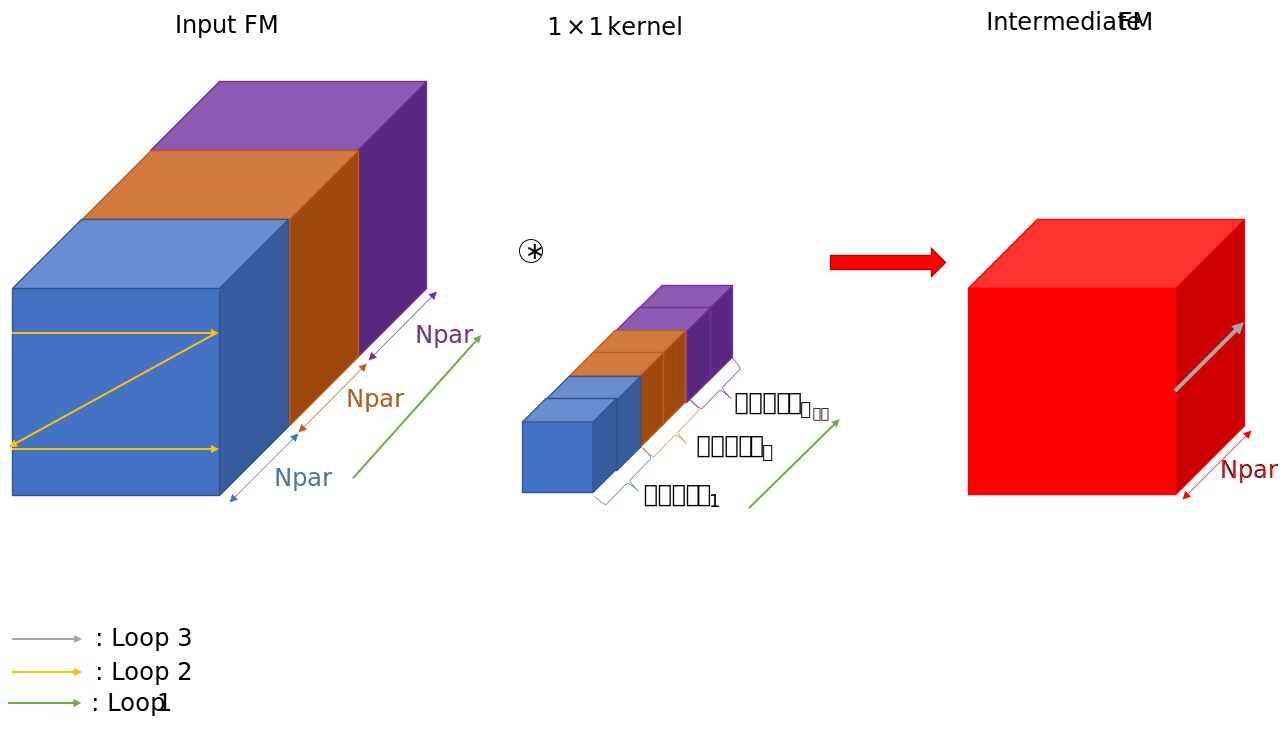
\includegraphics[width=\linewidth]{algo_c11.pdf}
        \caption{representation of the sparse $1 \times 1$ convolution}
        \label{fig:algo_11conv}
    \end{figure}
    %
    \item \textbf{\acrshort{dsc}} Once the $1 \times 1$ convolution has produced the next $N_{par}$ input channels of the \acrshort{dsc}, we can first do the depthwise convolution on the intermediate \acrshort{fm}. Once the depthwise convolution is done, we can fetch the corresponding weight fetching group in each of the pointwise filters and compute the partial results for each of the output \acrshort{fm}. The corresponding pseudocode is found in Algorithm \ref{pseudocode:dsc} and the process is shown in Figure \ref{fig:algo_dsc}.
    %
    \begin{algorithm}[H]
        \centering
        \begin{algorithmic}
            \For{$int_{f}:=0$; $int_{f} < N_{par}$; $int_{f}++$} \Comment{Loop 3}
                \For{$int_{x}:=0$; $int_{x} < N_{ix}$; $int_{x}++$} \Comment{Loop 2}
                    \For{$int_{y}:=0$; $int_{y} < N_{iy}$; $int_{y}++$} \Comment{Loop 2}
                        \For{$group:=0$; $group < N_{gr}$; $group++$} \Comment{Loop 1}
                            \For{$i_f:=0$; $i_f < N_{np}$; $i_f++$} \Comment{Unrolled}
                                \State{$wgt$  = $filter_{1 \times 1}$[$group_{int} \times N_{par} + int_f$][$group \times N_{par} + i_f$]}
                                \State{$acti$  = $FMI_{I}$[$wgt[pos] + group \times N_{par}$][$int_y$][$int_x$]}
                                \State{FM$_{int}$[$group_{int} \times N_{par} + int_f$][$int_y$][$int_x$]  += $acti \times wgt[val]$}
                            \EndFor
                        \EndFor
                    \EndFor
                \EndFor
            \EndFor
        \end{algorithmic}
        \caption{Sparse \acrshort{dsc} convolution pseudocode}
        \label{pseudocode:dsc}
    \end{algorithm}
    %
    \begin{figure}[H]
        \centering
        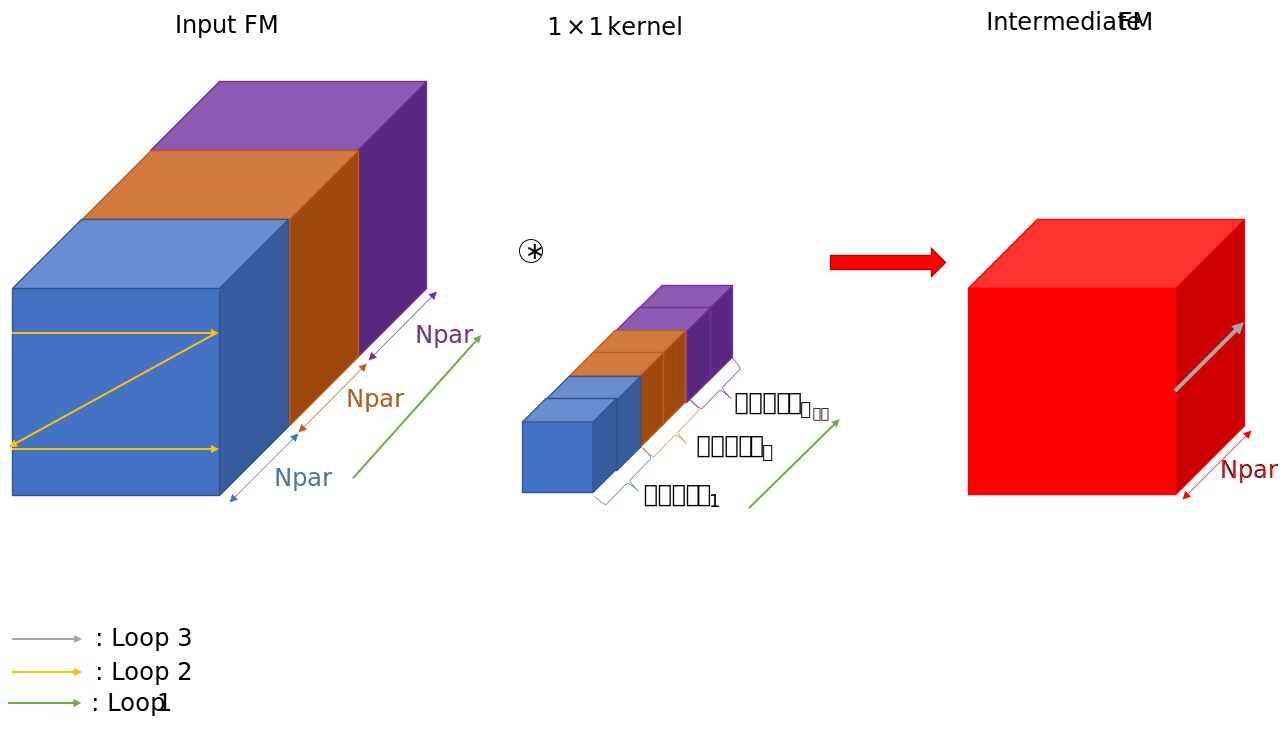
\includegraphics[width=\linewidth]{algo_c11.pdf}
        \caption{representation of the sparse \acrshort{dsc} convolution}
        \label{fig:algo_11conv}
    \end{figure}
\end{enumerate}
%
\subsection{Loop analysis}
%
Once we have determined how the convolutions is going to be performed
on \acrshort{fpga}, now we have to analyse the loop in order to find the optimal tiling, unrolling and loop interchange parameters.
%
%
\section{Implementing sparse DSC on FPGA} \label{sec:implementation}
In the previous section, we detailed how to prune $1 \times 1$ kernels, how the convolution process is performed, and we analyzed the design hardware variables. In this section, we explore how we can implement the chosen design into an \acrshort{fpga}. The hardware design was implemented using SystemVerilog and the corresponding code can be found at this address: \url{https://github.com/ggheysen/UCL-EPL-Master-Thesis-2019-2020}.

According to the scope of this thesis, the purpose of the implementation is to verify the fourth and fifth design objectives, namely:
%
\begin{itemize}
    \item The proposed architecture provides a logically correct output.
    \item An increase of the sparsity improves the performance of the architecture.
\end{itemize}
%
Those design objectives are related to the implementation of the inverted residual block with sparse $1 \times 1$ convolution. Therefore, instead of implementing each type of layer of MobileNetV2, we focus only on this one. As those two objectives are independent of the degree of parallelization, it was chosen to set all unrolling parameters to 1. We did not implement the skip connection since it is independent of the pruning scheme. However, as demonstrated by \textcite{bai_cnn_2018, liu_fpga-based_2019}, we can extend the convolution \acrshort{pe}s to support all kind of layers of MobileNetV2.

The performance results of the architecture will be discussed in next section. First, we describe the overall architecture in Section \ref{subsec:overal}, and then we go deeper into each component defined in the overall architecture. The architecture is inspired by three works: \textcite{zhu_efficient_2020, kang_accelerator-aware_2020, bai_cnn_2018}.
%
\subsection{Overall architecture} \label{subsec:overal}
%
The overall architecture has been inspired by \textcite{zhu_efficient_2020}. The mains components that compose our \acrshort{fpga}-based architecture are the following:
%
\begin{itemize}
    \item \textbf{External Memory}: it contains the \acrshort{cnn} data and it is where the output \acrshort{fm} will be stored.
    \item \textbf{Main controller}: it synchronizes the different components of the architecture by sending them control signals.
    \item \textbf{\acrfull{dma}}: it handles the read and write requests between the \acrshort{fpga} and the external memory.
    \item \textbf{\acrshort{pe}}: each \acrshort{pe} performs the actual convolution with the weight and pixel fetched from external memory into the on-chip memory. In the architecture, we have two kinds of \acrshort{pe}: $1 \times 1$ convolution \acrshort{pe} and \acrshort{dsc} \acrshort{pe}.
    \item \textbf{Buffer}: it composes the on-chip memory and contains a tile of data. There are two categories of buffer: \textbf{data buffer} which contains data from external memory and is read by the \acrshort{pe} and \textbf{result buffer} which is filled by \acrshort{pe}s and is read either by other \acrshort{pe} or by the \acrshort{dma} to write its content to external memory. There are four data buffers ($FM_{I}$ buffer, $Conv_{1 \times 1}$ buffer, $Conv_{DW}$ buffer, $Conv_{PW}$ buffer) and two result buffers ($FM_{int}$ buffer, $FM_{O}$ buffer).
\end{itemize}
%
\begin{figure}
    \centering
    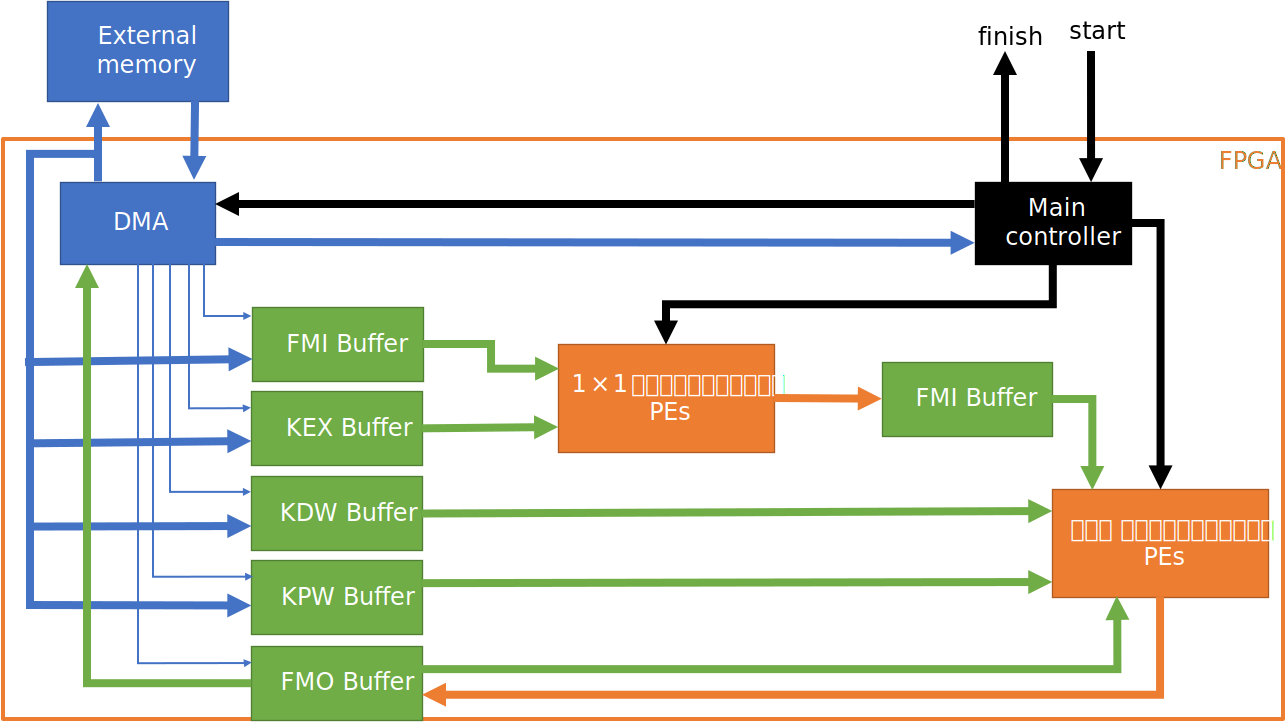
\includegraphics[width=\textwidth]{overal_archi.pdf}
    \caption{overall architecture of the accelerator}
    \label{fig:overal_archi}
\end{figure}
%
An illustration of the overall architecture can be found in Figure \ref{fig:overal_archi}. We should add that every component is synchronous with the clock signals and has reset signals. For the sake of clarity, this was not included in the drawing.

In the following sections, we will go into details about each component. An exhaustive list of the different input and output signals of each component can be found in Appendix \ref{appendix:sig}.
%
\subsection{External memory}
%
The external memory is an external component that contains all the data required to run the network (MobileNetV2) on an input \acrshort{fm}. Each data stored in the external memory can be identified by its address in the external memory. We can identify 5 types of data:
%
\begin{enumerate}
    \item \textbf{Input \acrshort{fm}}: the input \acrshort{fm} of a layer, where bitwidth representing one pixel is equal to $BW_{pixel}$. Channels are stored one by one, and the content of one channel is stored line by line. For example, the memory address of the pixel at position $\left(ix, iy, if\right)$ can be expressed using Equation \eqref{eq:addr_fmi}.
    \begin{equation}
        address_{FM_{I}}(ix, iy, if) = ix + iy \times N_{ix} + if \times N_{ix} \times N_{iy}
        \label{eq:addr_fmi}
    \end{equation}
    \item \textbf{Output \acrshort{fm}}: the output \acrshort{fm} is stored in the same manner as the input \acrshort{fm}. We should add that the output \acrshort{fm} of one layer becomes the input \acrshort{fm} of the next layer. Therefore, the addresses where the output \acrshort{fm} pixels are stored become the addresses of the input \acrshort{fm} of the next layer and inversely.
    %
    \item \textbf{$1 \times 1$ kernels}: the weights of the $1 \times 1$ convolution, where $BW_{weight}$ is the number of bits to represent the value of a weight and $log_2(N_{par})$ the number of bits to represent its position. Each $1 \times 1$ filter is stored kernel by kernel, and each kernel is stored weight by weight. For example, the memory address of the weight $x$ in fetching group \textquote{$group$} of kernel $f$ can be expressed using Equation \eqref{eq:addr_c11}.
    This terminology is used for weights from the $1 \times 1$ convolution from the bottleneck convolution and also from the $1 \times 1$ convolution layer.
    %
    \begin{equation}
        address_{K_{EX}}(kx, group, kf) = kx + group \times N_{np} + kf \times N_{np} \times N_{gr}
        \label{eq:addr_c11}
    \end{equation}
    \item \textbf{Depthwise kernels}: the depthwise kernels, where the bitwidth representing one weight is equal to $BW_{weight}$. Channels are stored one by one, and the content of one channel is stored line by line. For example, the memory address of the weigth at position $\left(kx, ky, kf\right)$ can be expressed using Equation \eqref{eq:addr_dw}.
    \begin{equation}
        address_{K_{DW}}(kx, ky, kf) = kx + ky \times N_{kx} + kf \times N_{kx} \times N_{ky}
        \label{eq:addr_dw}
    \end{equation}
    \item \textbf{Pointwise kernels}: the kernels of the pointwise convolution. The weights are stored in the same manner as for the $1 \times 1$ filter.
    \item \textbf{Standard convolution kernels}: since the first layer of MobileNetV2 is a standard convolution \cite{sandler_mobilenetv2_2019}, the weights must be also stored in the external memory, in the same manner as the depthwise filter.
\end{enumerate}

An offset, for each type of data, is added to the computation of the address to avoid that one address is shared between multiple data. As a result, before executing one layer, the main controller must have the following information, labelled as \textbf{Layer information}:
%
\begin{enumerate}
    \item \textbf{$N_{ix}$ and $N_{iy}$}: the spatial dimensions of the input \acrshort{fm}. Since $N_{ix}, N_{iy} \leq 224$ \cite{sandler_mobilenetv2_2019}, we can use 8 bits to represent them.
    \item \textbf{$N_{if}$ and $N_{of}$}: the number of channels of the input  and output \acrshort{fm}. Since $N_{if}, N_{of} \leq 1280$ \cite{sandler_mobilenetv2_2019}, we can use 11 bits to represent them.
    \item \textbf{$t$}: the expansion factor of the $1 \times 1$ convolution. Since $t \leq 6$ \cite{sandler_mobilenetv2_2019}, we can use 3 bits to represent it.
    \item \textbf{$S$}: the value of the stride. Since $S$ can be either 1 or 0 \cite{sandler_mobilenetv2_2019}, we can use 1 bit to represent it.
    \item \textbf{$N_{gr}$ and $N_{grint}$}: the number of fetching groups for the $1 \times 1$ convolution and the \acrshort{dsc}. Since the largest value possible for both parameters is the maximum $N_{if}$ ($N_{par} = 1$), we can use 11 bits to represent them.
    \item \textbf{$Layer$}: to tell the main controller which layer is going to be executed. Since there are 4 kinds of layers in MobileNetV2 \cite{sandler_mobilenetv2_2019}, we use 2 bits to represent it. However this was not included in the design because only the bottleneck convolution was implemented.
    \item \textbf{Offsets}: the offset of the different data types must be transfered to the \acrshort{dma} in order to correctly compute the address of the required data. The number of bits required to represent one offset is the bitwidth of the address of the external memory.
\end{enumerate}

%
\begin{figure}
    \centering
    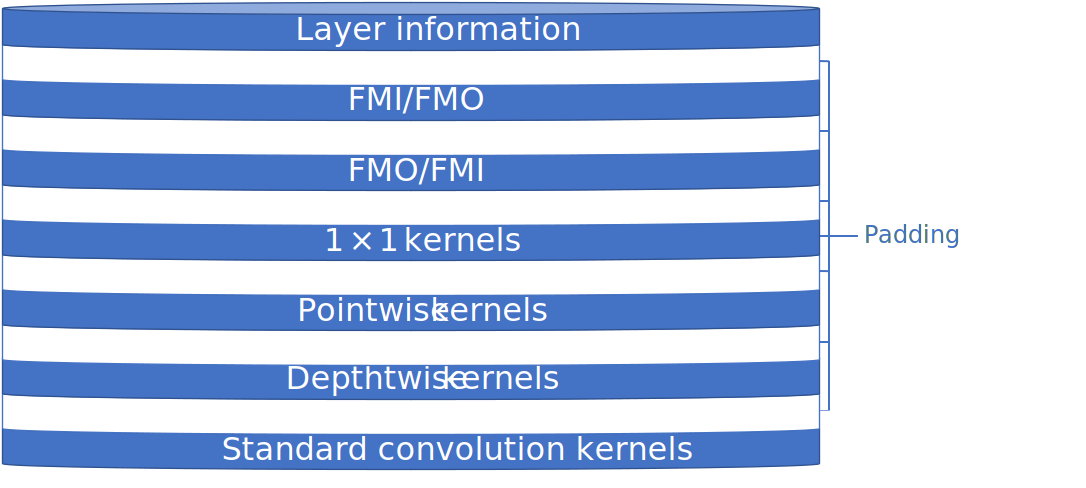
\includegraphics[width=\textwidth]{overal_mem.pdf}
    \caption{overall structure of the external memory}
    \label{fig:overal_mem}
\end{figure}
%
As a consequence, those layer information are also stored in the external memory. The overall structure of the external memory can be found in Figure \ref{fig:overal_mem}.
%
\subsection{Main controller}
%
The role of the main controller is to synchronize the different components of the architecture (except the memory components). Therefore, each component is a \textquote{slave} that stays in an idle state until the main controller wakes up one of them to perform a particular operation.

To wake up a component, the main controller sends it a starting signal $s_{*}$ and optionnaly additional information about the operation to perform. Afterwards, the main controller remains idle, waiting for the component to terminate its operation. Once the component has completed its task, it sends a finishing signal $f_{*}$ to the main controller.

The main controller remains in an idle state until it receives a starting signal indicating that the external memory contains all data to perform a bottleneck convolution. I have implemented the main controller to compute one bottleneck convolution, but its architecture could be extended to iterate through all the layers of the network.

%
\begin{figure}
    \centering
    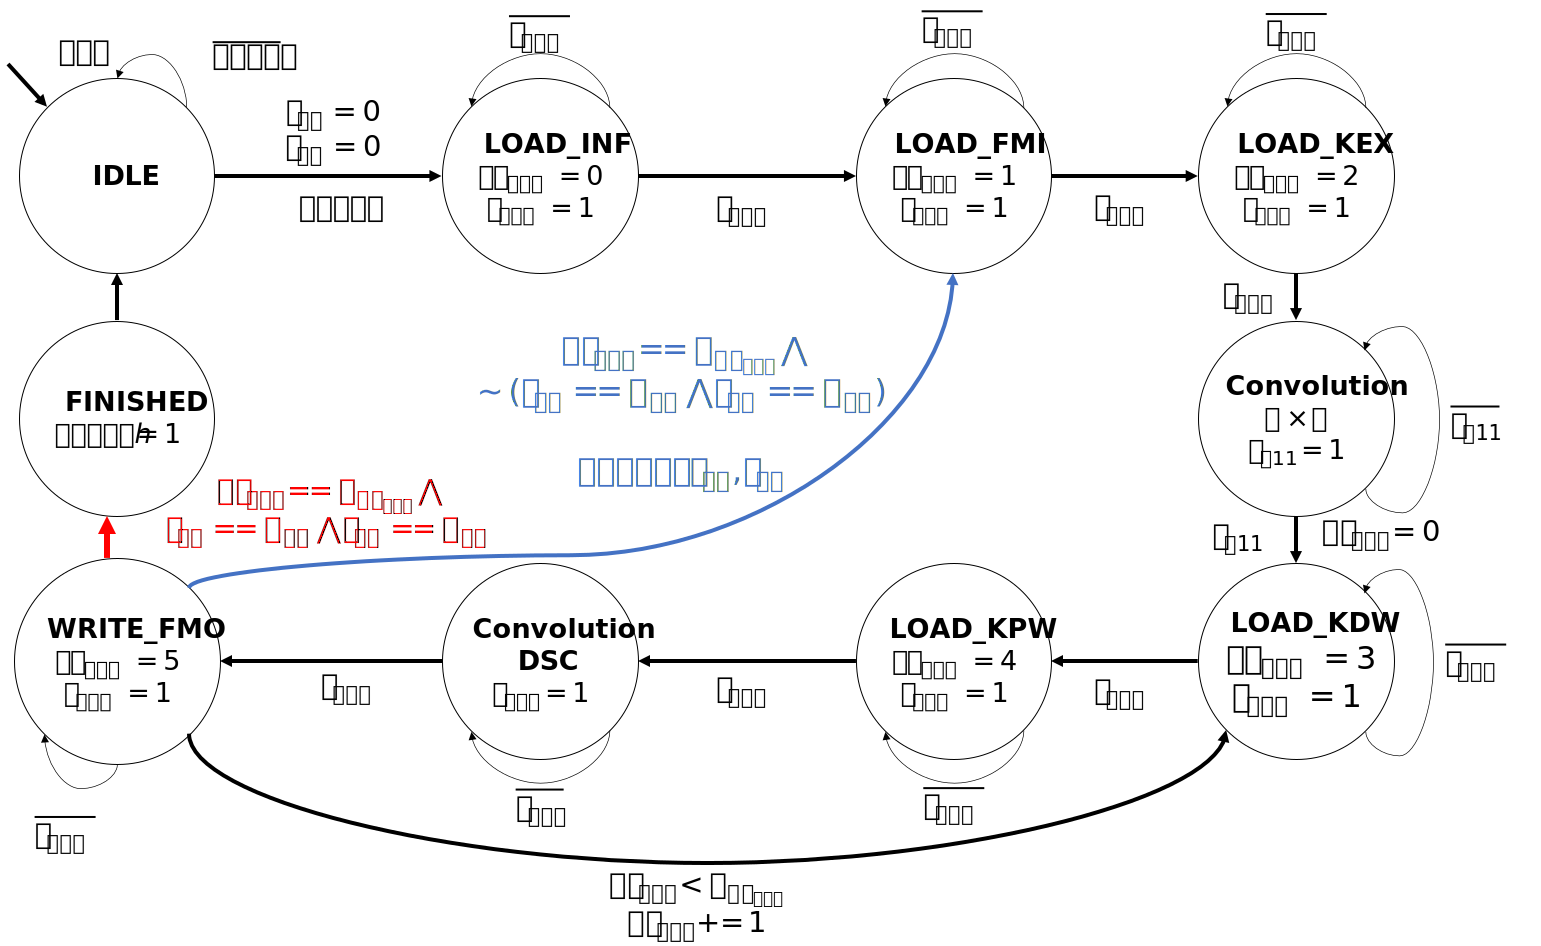
\includegraphics[width=\textwidth]{fsm-mc.pdf}
    \caption{\acrshort{fsm} of the main controller}
    \label{fig:fsm_mc}
\end{figure}
We can describe the behavior of the main controller using a \acrfull{fsm}, as illustrated in Figure \ref{fig:fsm_mc}. The \textbf{IDLE} state is the state where the main controller is waiting to perform a bottleneck convolution. Once the main controller has received a starting signal, it performs the following operations:
%
\begin{figure}
    \centering
    %
    \begin{subfigure}[t]{.49\textwidth}
        \centering
        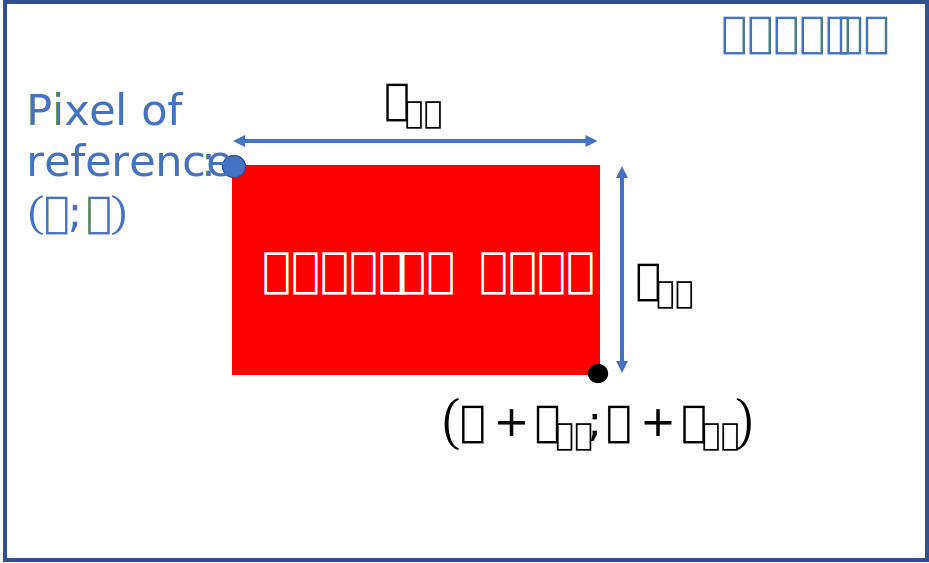
\includegraphics[width=\linewidth]{pixofref.pdf}
        \caption{Example of pixel of reference for an input \acrshort{fm} tile}
        \label{fig:pix_of_ref}
    \end{subfigure}
    %
    \begin{subfigure}[t]{.49\textwidth}
        \centering
        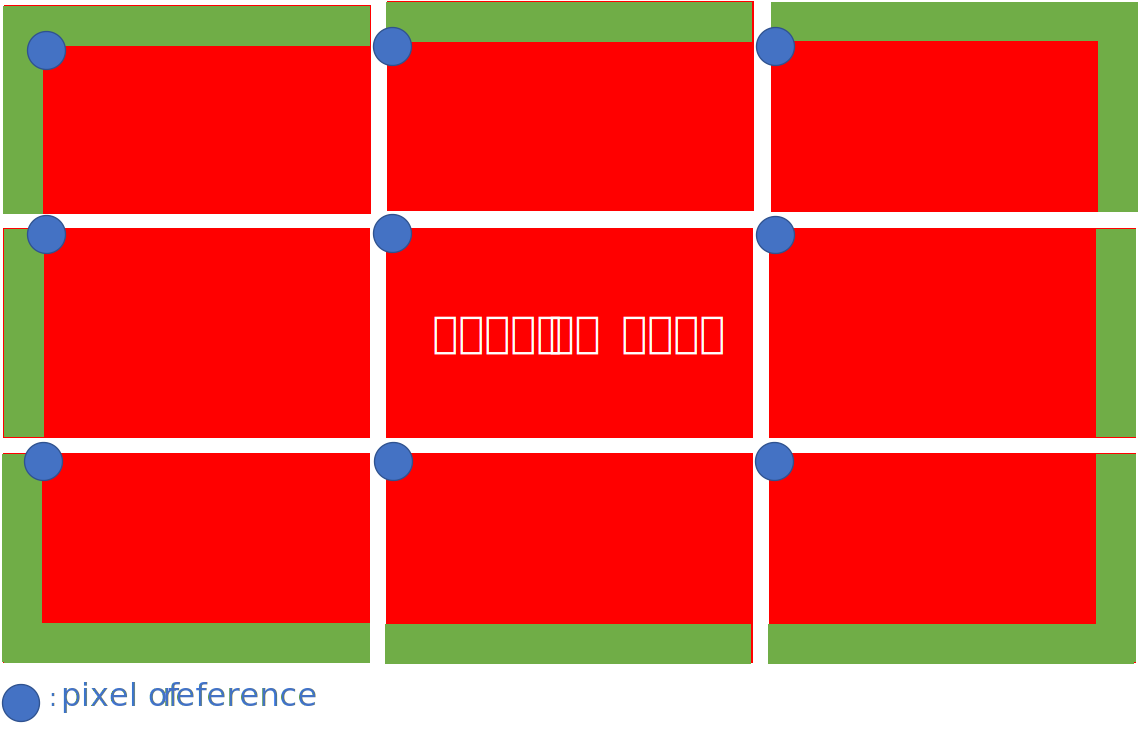
\includegraphics[width=\linewidth]{tilepadding.pdf}
        \caption{Padding configuration of input \acrshort{fm} tiles, where red area represent pixels fetched from external memory and green area represent padding pixels}
        \label{fig:tile_padding}
    \end{subfigure}
    %
    \caption{Illustration of the concept of pixel of reference and padding}
\end{figure}
%
\begin{enumerate}
    \item \textbf{LOAD\_INF}: to perform the bottleneck convolution, the main controller first needs to fetch the layer information stored in the external memory. Therefore it tells the \acrshort{dma} to fetch them.
    %
    \item \textbf{LOAD\_FMI}: the bottleneck convolution starts by fetching a tile of inputs and weights from the main memory. As all inputs in the channel-axis are buffered (corresponding to all the fetching groups), an input \acrshort{fm} tile can be determined only by the spatial coordinates of the tile first element - pixel of reference (with the smallest $(x, y)$). Indeed, the \acrshort{dma} can fetch, for each channel, all pixels in the range $[(x, y); (x+T_{ix}, y+T_{iy})]$, which corresponds to the tile, as illustrated in Figure \ref{fig:pix_of_ref}. As a result, when the main controller asks the \acrshort{dma} to load into the on-chip memory a tile of input \acrshort{fm}, it also transfers the spatial coordinates and the memory address of its pixel of reference. Moreover, since we have to add padding to the tile (spatial dimensions are not reduced by the convolution operations), 0 value pixels are stored in the on-chip memory at corresponding positions when the reference pixel is on one edge of the input \acrshort{fm}, as shown in Figure \ref{fig:tile_padding}.
    %
    \item \textbf{LOAD\_KEX}: after fetching the input \acrshort{fm} tile, the main controller asks the \acrshort{dma} to load the $N_{par}$ $1 \times 1$ kernels into the on-chip memory, corresponding to the intermediate fetching group $group_{int}$. %Rajouter le channel de ref
    \item \textbf{CONV\_11}: after loading the weights and pixels, the $1 \times 1$ convolution can be performed. Once the $N_{par}$ intermediate channels corresponding to the intermediate fetching group $group_{int}$ have been produced, the \acrshort{dsc} can be executed.
    \item \textbf{LOAD\_KDW} and \textbf{LOAD\_KPW}: before doing the \acrshort{dsc}, the pointwise and depthwise kernels corresponding to the intermediate fetching group should be loaded.
    \item \textbf{CONV\_DSC}: all output \acrshort{fm} tile partial products can be computed by performing the \acrshort{dsc} on the $N_{par}$ intermediate channels. If all intermediate fetching groups have been processed, final results are computed and can be written into the external memory. Otherwise, the next $N_{par}$ intermediate channels should be computed. Moreover, since output \acrshort{fm} partial results will be kept in on-chip memory, the main controller indicates to the \acrshort{dsc} \acrshort{pe}s whether the values read from the \textit{FMO Buffer} should be consired as valid. If it is not the case, the value should be set to 0.
    \item \textbf{WRITE\_FMO}: this state indicates that there are only final results in the \textit{FMO Buffer}. The main controller tells the \acrshort{dma} that its content can be written to the external memory. As for the input \acrshort{fm} tiles, the output \acrshort{fm} tiles are determined by their pixel of reference, which is also transmitted to the \acrshort{dma}. If all tiles have been processed, the bottleneck convolution is completed and the main controller state turns to \textbf{FINISHED}. Otherwise, a new tile has to be processed and main controller returns to \textbf{LOAD\_FMI} state.
    \item \textbf{FINISHED}: The bottleneck convolution is done and the main controller sets the finish signal.
\end{enumerate}
%
\subsection{DMA}
%
The purpose of the \acrshort{dma} is to fill the \textbf{data buffer} with its corresponding tile fetched from external memory and write the output pixels into the external memory. Therefore, it has to manage six types of operation, referenced by its operation number $op_{dma}$:
%
\begin{itemize}
    \item $op_{dma} = 0$: Load the layer information
    \item $op_{dma} = 1$: Load an input \acrshort{fm} tile, referenced by its pixel of reference. The \acrshort{dma} needs as extra information the coordinate and the memory address of that pixel of reference.
    \item $op_{dma} = 2$: Load the $1 \times 1$ kernels used to produce the intermediate fetching group $group_{int}$ of size $N_{par}$. The \acrshort{dma} needs as extra information the first kernel and the memory address of its first weight to correctly load the $N_{par}$ kernels.
    \item $op_{dma} = 3$: Load the depthwise kernels corresponding to the intermediate fetching group $group_{int}$ of size $N_{par}$. The \acrshort{dma} needs as extra information the first kernel of the group and the memory address of its first weight to correctly load the $N_{par}$ kernels.
    \item $op_{dma} = 4$: Load the weight fetching group (of size $N_{np}$) of all pointwise kernels corresponding to the intermediate fetching group $group_{int}$. The \acrshort{dma} needs as extra information the position of the first weight in the fetching group and its memory address.
    \item $op_{dma} = 5$: Write the content of the \textbf{FMO Buffer} into the external memory, which corresponds to a tile of output \acrshort{fm}. As this tile is referenced by its pixel of reference, the \acrshort{dma} needs as extra information the coordinate and the memory address of that pixel of reference.
\end{itemize}

%
\begin{figure}
    \centering
    
\includegraphics[width=\textwidth]{fsm-dma.pdf}
    \caption{\acrshort{fsm} of the \acrshort{dma}}
    \label{fig:fsm_dma}
\end{figure}
When the main controller asks the \acrshort{dma} for a transfer, it sets its start signal, which operation to execute ($op_{dma}$), and all extra information required. All extra information are related to the external memory, if the \acrshort{dma} reads or writes into a buffer, the initial address $r_{addr-i}/w_{addr-i}$ can be set to 0. The behavior of the \acrshort{dma} can be expressed using a \acrshort{fsm}, as found in Figure \ref{fig:fsm_dma}. A general \acrshort{fsm} has been illustrated because each operation shares the same structure. As the \acrshort{dma} only fetches data from one memory and writes the data into another one, each operation is composed of 2 states:
\begin{itemize}
    \item \textbf{READ}: the \acrshort{dma} fetches the required data at a address $r_{addr}$. Once the data is loaded by the \acrshort{dma}, it moves to the next state to write the data in the on-chip memory. When loading the input \acrshort{fm} tile, if the address corresponds to a padding pixel, the value to write is 0 and the \acrshort{dma} directly moves to the \textbf{WRITE} state. If the data is fetched from the external memory, the \acrshort{dma} waits the data read from the external memory to be valid. But if the data is fetched from a buffer, the process can be pipelined. That is why, before the \acrshort{dma} reads data from the on-chip memory, it is in a state called \textbf{RAM\_LOADING} to initialize the pipeline process.
    \item \textbf{WRITE}: the \acrshort{dma} sends a write signal and the associated data $w_data$ and address $w_{address}$ to the corresponding memory . If the operation is finished (the tile has been fetches), the \acrshort{dma} goes into the \textbf{FINISHED} state. Otherwise, it updates the address of the next data to fetch and goes back to the \textbf{READ} state.
\end{itemize}

Since the \acrshort{dma} performs one transfer at a time, we can share the fetched data (to be written) $w_{data}$ between all memory component and we set the write signal to the corresponding component. In a similar way, the signal to access or write data in a buffer $ram_{addr}$ can also be shared between the different buffers.
%
\subsection{1\texttimes1 convolution PE}
%
The purpose of this component is to execute the Algorithm \ref{fig:algo_11conv}. The behavior of the \acrshort{pe} can be expressed using a \acrshort{fsm}, as found in Figure \ref{fig:fsm_c11}.

When the \acrshort{pe} receives a starting signal, it means that the \textbf{FMI} and \textbf{KEX BUFFERS} contain the data to execute the next $1 \times 1$ convolution. For each fetching group corresponding to an intermediate pixel at address $\left( int_x, int_y, int_f \right)$, the \acrshort{pe} loads the corresponding inputs and weights into its registers (\textbf{LOAD\_DATA} state). Once it is done, the computation can be performed (\textbf{COMPUTATION} state). Since the convolution is fully-unrolled, an exemple of the hardware configuration is shown in Figure \ref{fig:c11_hardware}. The output result is then summed with the content of the accumulator (which contains 0 for the first fetching group).

When the convolution is done for one intermediate pixel, the result is written into the \textbf{FMINT BUFFER}. If all pixels required for the \acrshort{dsc} have been computed, the \acrshort{pe} sends an ending signal to the main controller (\textbf{FINISHED} state). Otherwise it computes the next intermediate pixel.
%
\subsection{DSC PE}
%
This \acrshort{pe} is designed to perform the \acrshort{dsc}. Once the $1 \times 1$ convolution has computed the next \acrshort{dsc} fetching group and the \textbf{Buffers} containts the required data, we can do the \acrshort{dsc} as in Algorithm \ref{fig:algo}. The \acrshort{pe} can be described as a \acrshort{fsm} executign Algorithm \ref{fig:algo_dsc}.
%
\subsection{Buffer}
%
\begin{figure}
    \centering
    
\includegraphics[width=\textwidth]{struct_ram.pdf}
    \caption{General architecture of a buffer component}
    \label{fig:struct_ram}
\end{figure}
%
The buffers compose the on-chip memory of the \acrshort{fpga}. As mentionned previously, the structure is composed of six buffers that share the same structure, as illustrated in Figure \ref{fig:struct_ram}. At each clock period, the output signal $res$ is equal to the value stored at address $addr$, or if the write signal $write$ is enabled, the value that is currently written. In the same way, if the write signal is set, the value in the buffer at address $addr$ is equal to the input data $w_{data}$. As multiple components may read or write a same buffer, a multiplexer is added to select from which address to read.

The value of $addr_r$ and $addr_w$ depend on the type of buffer. For \textbf{data buffer} the $addr_r$ is the \acrshort{pe} address of the corresponding buffer, and $addr_w$ is the \acrshort{dma} $ram_{addr}$ signals. For \textbf{result buffer}, $addr_w$ is the corresponding \acrshort{pe} output address and $addr_r$ can be either a \acrshort{pe} address requesting a result (\textbf{FMINT Buffer}) or the \acrshort{dma} $ram_{addr}$ signals to write final results to external memory ((\textbf{FMO Buffer}))

However, the differences between each buffer are the maximum number of elements that can be stored $N_{elem}$ and the bitwidth $BW$ of their data stored. We explore for each buffer these two parameters.
\begin{itemize}
    \item \textbf{FMI Buffer}: we have determined from the loops analysis that we buffer each input \acrshort{fm} fetching group. Since the number of input \acrshort{fm} channels vary accross the different layers of the network, we can determine $N_{elem}$ using Equation \eqref{eq:nelem-fmi}. The number of bits to store a pixel is equal to $BW_{pixel}$. We can therefore express $BW$ such as Equation \eqref{eq:bw-fmi}.
    \begin{equation}
        N_{elem-fmi} = \forall l \in layers: Max\left( N_{if}^l \times Min\left(T_{ix}, N_{ix}^l\right) \times Min\left(T_{iy}, N_{iy}^l\right) \right)
        \label{eq:nelem-fmi}
    \end{equation}
    \begin{equation}
        BW_{fmi} = BW_{pixel}
        \label{eq:bw-fmi}
    \end{equation}
    %
    \item \textbf{KEX Buffer}: this buffer stores the $N_{par}$ $1 \times 1$ kernels required to perform this convolution, which expands the number of input channels. Therefore, we can express $N_{elem}$ using Equation \eqref{eq:nelem_kex}, where $N_{gr-max} = \left\lceil \frac{1280}{Npar} \right\rceil$ is the maximum number of fetching group in the whole network. Since the weights are expressed in the proposed compressed format, we also have to store the weight position in the fetching group.
    As a result, $BW$ can be expressed using Equation \eqref{eq:bw-kex}, where $BW_{weight}$ is the number of bits to represent a weight and $log_2(N_{par})$ the number of bits to represent the position.
    \begin{equation}
        N_{elem-kex} = N_{par} \times N_{np} \times N_{gr-max}
        \label{eq:nelem_kex}
    \end{equation}
    \begin{equation}
        BW_{kex} = BW_{weight} + log_2(N_{par})
        \label{eq:bw-kex}
    \end{equation}
    %
    \item \textbf{FMINT Buffer}: since the \acrshort{dsc} needs $N_{par}$ intermediate \acrshort{fm} channels and the $1 \times 1$ convolution does not reduce the spatial dimension of the input \acrshort{fm}, we can express the $N_{elem}$ using Equation \eqref{eq:nelem_fmint}. The bitwidth of a pixel is the bitwidth used to represent a pixel, as in Equation \eqref{eq:bw-fmint}.
    \begin{equation}
        N_{elem-fmint} = N_{par} \times T_{iy} \times T_{ix}
        \label{eq:nelem_fmint}
    \end{equation}
    \begin{equation}
        BW_{fmi} = BW_{pixel}
        \label{eq:bw-fmint}
    \end{equation}
    %
    \item \textbf{KDW Buffer}: applying the same methodoly as \textbf{FMINT Buffer} and since the depthwise kernels are fully buffered, we can express the $N_{elem}$ using Equation \eqref{eq:nelem_kdw}. The bitwidth of a pixel is the bitwidth used to represent a weight, as in Equation \eqref{eq:bw-kdw}.
    \begin{equation}
        N_{elem-kdw} = N_{par} \times N_{ky} \times N_{kx}
        \label{eq:nelem_kdw}
    \end{equation}
    \begin{equation}
        BW_{kdw} = BW_{weight}
        \label{eq:bw-kdw}
    \end{equation}
    %
    \item \textbf{KPW Buffer}: for each time we perform a \acrshort{dsc}, we need to convolve in each pointwise the corresponding weight fetching group with $N_{np}$ pixels in the $N_{par}$ channels. The maximum number of elements in the buffer can be computed using Equation \eqref{eq:nelem_kpw}. As the pointwise convolution is a $1 \times 1$ convolution, the bitwidth associated to each pointwise kernel is the same as the \textbf{KPW Buffer}, and can be expressed using Equation \ref{eq:bw-kpw}
    \begin{equation}
        N_{elem-kpw} = N_{np} \times N_{of}
        \label{eq:nelem_kpw}
    \end{equation}
    \begin{equation}
        BW_{kpw} = BW_{weight} + log_2(N_{par})
        \label{eq:bw-kpw}
    \end{equation}
    %
    \item \textbf{FMO Buffer}: using the same methodoly as for determining $N_{elem}$ and $BW$ for the \textbf{FMI Buffer}, they are expressed using Equation \eqref{eq:nelem_fmo} and \eqref{eq:bw_fmo}
    \begin{equation}
        N_{elem-fmo} = \forall l \in layers: Max\left( N_{of}^l \times Min\left(T_{oy}, N_{oy}^l\right) \times Min\left(T_{ox}, N_{ox}^l\right) \right)
        \label{eq:nelem_fmo}
    \end{equation}
    \begin{equation}
        BW_{fmo} = BW_{pixel}
        \label{eq:bw_fmo}
    \end{equation}
\end{itemize}

%

%
%
\chapter{Measure and Results}
blabla
%
%
\afterpage{\blankpage}
\cleardoublepage
\newpage
